\section{Final Evaluated Local Correction and Memory Study}
\label{sec:final-evaluation}
\subsection{Completed population, method, and evaluation}
The independent R85 study completes 520 of 520 outputs with successful automatic evaluation on 40 sources, four per official category. Six arms use seeds 0 and 17; deterministic RF-Edit I08 uses seed 0 once per source. The source is the statistical unit: we average seeds within each source and give sources equal weight. The primary method is TraceMemory (CORR25); BOTH25 is the preregistered secondary spatial-memory configuration. R84 provides the separate seen-source dose study: all 130 outputs from ten sources completed automatic evaluation. Development and independent populations are not pooled.

The method uses only source and target prompts to construct $E$ and $P=1-0.75E$. Official edit annotations enter evaluation only. The primary correction is $0.25P\odot c_i$ without RMS restoration. Its first-seven-step full-source, all-query memory is unchanged. BOTH additionally pools $P$ to the packed image-query grid. ENERGY uses Eq.~\eqref{eq:energy-control}, preserving the global residual direction at the local rule's same-state RMS. These three arms each cost 97 standalone NFE, including six native probe calls.

Target and directional CLIP use ViT-L/14; DINO uses full-image DINOv2-base cosine similarity. AlexNet LPIPS is reported for the whole image and as a spatial-map average weighted by the area-resampled official preservation complement. LPIPS feature receptive fields can cross that boundary. All 40 sources contribute full-image metrics; preservation metrics use 33 sources, with seven empty complements omitted. R84 analogously uses ten full-image and eight preservation-eligible sources. Full-image source distance includes requested changes, so preservation LPIPS is the regional retention comparison.

\begin{table*}[t]
\centering\small
\caption{Final R85 evaluation: equal-source means on 40 independent sources and seven methods. CLIP target, directional CLIP, and full-image DINO are higher-is-better; LPIPS is lower-is-better. Preservation LPIPS uses 33 sources. Six arms have 80 outputs each; RF-Edit has 40. NFE is the complete standalone transformer-call count.}
\label{tab:final-means}
\setlength{\tabcolsep}{5pt}
\begin{tabular}{lrrrrrr}
\toprule
Method & CLIP target $\uparrow$ & CLIP dir. $\uparrow$ & DINO $\uparrow$ & LPIPS full $\downarrow$ & LPIPS preserved $\downarrow$ & NFE\\
\midrule
TraceMemory (CORR25) & 0.2629 & 0.0863 & 0.5904 & 0.5419 & 0.5142 & 97\\
BOTH25 (secondary) & 0.2733 & 0.1069 & 0.5579 & 0.5620 & 0.5269 & 97\\
ENERGY\_MATCH25 & 0.2622 & 0.0881 & 0.5856 & 0.5483 & 0.5226 & 97\\
U25\_KV & 0.2632 & 0.0908 & 0.6111 & 0.4971 & 0.4743 & 91\\
FlowEdit N26 & 0.2712 & 0.1177 & 0.5737 & 0.4437 & 0.4281 & 52\\
RF-Inversion ETA03 & 0.2694 & 0.1065 & 0.4670 & 0.5431 & 0.5322 & 56\\
RF-Edit I08 & 0.2453 & 0.0383 & 0.7875 & 0.2778 & 0.2688 & 100\\
\bottomrule
\end{tabular}
\end{table*}

\subsection{Source-paired estimates and localization benefit}
Pointwise percentile 95\% intervals use 10,000 source-bootstrap resamples. Two-sided source sign-flip tests use 10,000 Monte Carlo draws with plus-one correction. The planned Holm family contains six CORR25 comparisons separately within each metric, including BOTH and RF-Edit; Table~\ref{tab:final-paired} reports this adjusted $p$. RF-Edit's single deterministic result is compared with each other arm's two-seed source mean.

CORR25 reduces preservation LPIPS relative to ENERGY by 0.0084, with interval $[-0.0143,-0.0022]$ and adjusted $p=0.0238$. Full-image LPIPS decreases by 0.0064 ($p=0.0014$). This is a modest measured benefit from request-conditioned allocation beyond the global same-state magnitude control. Target CLIP differs by $+0.0007$ and directional CLIP by $-0.0018$, with intervals spanning zero; the target and directional CLIP intervals both span zero. Each arm evolves on its own trajectory, with its own cumulative correction energy.

\begin{table*}[t]
\centering\footnotesize
\caption{Selected final source-paired effects. Differences are first arm minus second. Intervals are pointwise 95\% source-bootstrap intervals; $p_{\rm H}$ uses six planned comparisons per metric. BOTH--CORR25 is the sign-reversed member of that family. Source counts are 33 for preservation LPIPS and 40 otherwise.}
\label{tab:final-paired}
\setlength{\tabcolsep}{5pt}
\begin{tabular}{llrrr}
\toprule
Comparison & Metric & Difference & 95\% interval & $p_{\rm H}$\\
\midrule
CORR25 $-$ ENERGY & LPIPS preserved & $-0.0084$ & $[-0.0143,-0.0022]$ & 0.0238\\
CORR25 $-$ ENERGY & LPIPS full & $-0.0064$ & $[-0.0098,-0.0030]$ & 0.0014\\
CORR25 $-$ ENERGY & Directional CLIP & $-0.0018$ & $[-0.0066,0.0030]$ & 0.5297\\
CORR25 $-$ FlowEdit & Directional CLIP & $-0.0315$ & $[-0.0504,-0.0137]$ & 0.0084\\
CORR25 $-$ FlowEdit & LPIPS preserved & $+0.0861$ & $[0.0500,0.1224]$ & 0.0006\\
CORR25 $-$ FlowEdit & DINO & $+0.0167$ & $[-0.0326,0.0704]$ & 1.0000\\
CORR25 $-$ U25 & LPIPS preserved & $+0.0399$ & $[0.0331,0.0469]$ & 0.0006\\
BOTH $-$ CORR25 & Target CLIP & $+0.0104$ & $[0.0054,0.0159]$ & 0.0006\\
BOTH $-$ CORR25 & Directional CLIP & $+0.0207$ & $[0.0099,0.0334]$ & 0.0012\\
BOTH $-$ CORR25 & LPIPS preserved & $+0.0127$ & $[0.0077,0.0180]$ & 0.0006\\
BOTH $-$ CORR25 & DINO & $-0.0325$ & $[-0.0591,-0.0109]$ & 0.0160\\
CORR25 $-$ ETA03 & DINO & $+0.1234$ & $[0.0700,0.1826]$ & 0.0010\\
\bottomrule
\end{tabular}
\end{table*}

\subsection{Benchmark position and memory trade-off}
FlowEdit N26 has higher directional CLIP and lower full-image and preservation LPIPS than CORR25, using 52 rather than 97 NFE. CORR25 minus FlowEdit gives directional CLIP $-0.0315$ ($p_{\rm H}=0.0084$) and preservation LPIPS $+0.0861$ ($p_{\rm H}=0.0006$). The DINO difference is $+0.0167$ with interval $[-0.0326,0.0704]$, leaving its direction uncertain. U25 has lower full-image and preservation LPIPS, higher mean DINO, and slightly higher CLIP means at 91 NFE. FlowEdit combines stronger directional CLIP with lower LPIPS and fewer evaluations; U25 also has lower LPIPS at fewer evaluations. CORR25 improves full-image DINO over RF-Inversion ETA03 by 0.1234 ($p_{\rm H}=0.0010$), while RF-Edit emphasizes retention with lower semantic alignment.

BOTH increases both semantic proxies: target CLIP increases by 0.0104 and directional CLIP by 0.0207 relative to CORR25. Preservation LPIPS increases by 0.0127, full-image LPIPS by 0.0201, and DINO decreases by 0.032496. Spatial memory attenuation therefore releases more prompt-driven change together with more source departure. The primary and secondary roles were fixed before the independent evaluation.

\begin{figure*}[t]
\centering
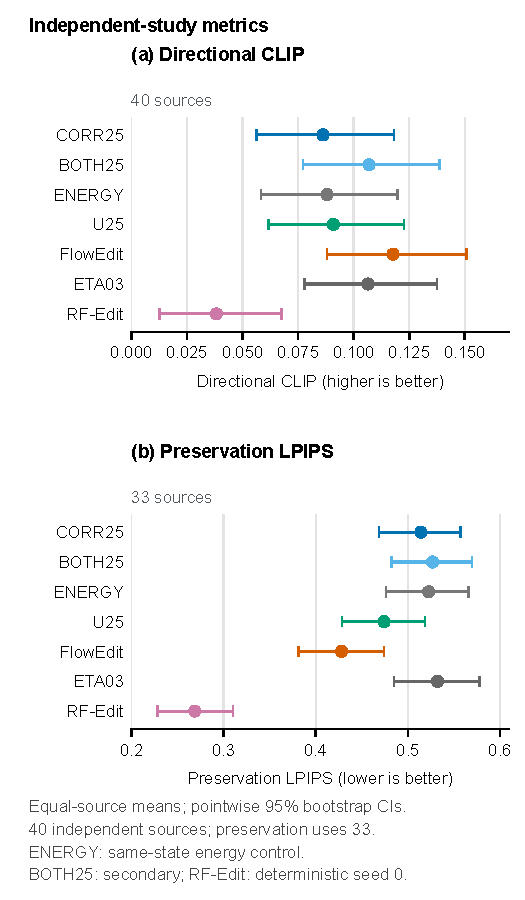
\includegraphics[width=.96\textwidth]{figures/final_metrics.pdf}
\caption{Final R85 metrics in a common arm order. The two horizontal-dot panels show source-level mean directional CLIP and preservation LPIPS with pointwise 95\% source-bootstrap intervals. Directional CLIP uses 40 sources; preservation LPIPS uses 33. Intervals describe each mean, while Table~\ref{tab:final-paired} reports paired differences.}
\label{fig:final-metrics}
\end{figure*}

\subsection{Development dose response and qualitative cases}
R84 evaluates the frozen direct local coefficients 0.15, 0.25, and 0.35 on ten seen sources (Table~\ref{tab:r84-dose}). Increasing correction strength lowers both full-image and preservation LPIPS. Relative to 0.15, CORR25 changes these metrics by $-0.0551$ and $-0.0561$; relative to 0.35, the differences are $+0.0473$ and $+0.0422$. All four comparisons have within-metric Holm $p\leq0.046875$. Target and directional CLIP difference intervals span zero in both dose comparisons. This development result identifies a preservation response to correction strength; the primary coefficient and BOTH's secondary role remain fixed for R85.

\begin{table*}[t]
\centering\small
\caption{R84 seen-source dose study. Means use ten sources for CLIP and DINO, eight for preservation LPIPS, and two seeds per source. Each arm costs 97 NFE. The complete R84 evaluation has 130 outputs including its other controls.}
\label{tab:r84-dose}
\begin{tabular}{lrrrrrr}
\toprule
Local coefficient & CLIP target & CLIP dir. & DINO & LPIPS full & LPIPS preserved & NFE\\
\midrule
0.15 & 0.2618 & 0.0964 & 0.5543 & 0.5827 & 0.5544 & 97\\
0.25 & 0.2609 & 0.0979 & 0.5946 & 0.5276 & 0.4983 & 97\\
0.35 & 0.2562 & 0.0939 & 0.6063 & 0.4803 & 0.4561 & 97\\
\bottomrule
\end{tabular}
\end{table*}

\begin{figure*}[t]
\centering
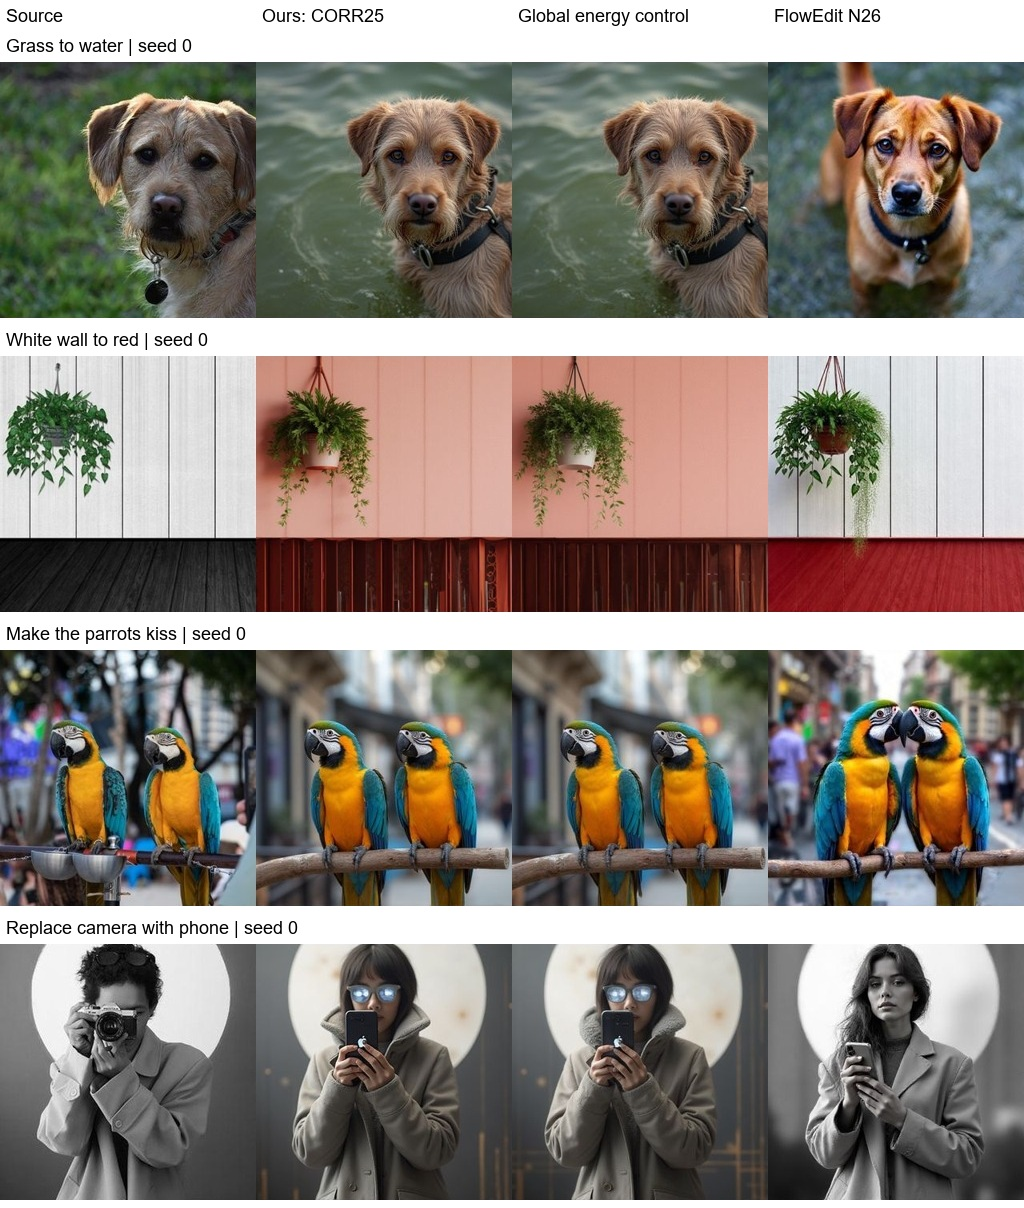
\includegraphics[width=.98\textwidth]{figures/final_qualitative.jpg}
\caption{Final seed-0 qualitative comparisons. Columns: source, TraceMemory (CORR25), ENERGY\_MATCH25, and FlowEdit. Rows show grass-to-water, wall-to-red, parrots-kissing, and camera-to-phone requests. The common examples expose appearance changes and requested relational or category changes alongside source retention; quantitative conclusions use the full source population.}
\label{fig:final-qualitative}
\end{figure*}
